
\vspace{1.0cm}

\subsection{Vertex detector}
\writer{Auguste Besson, Akimasa Ishikawa, Marcel Vos}{3}

The vertex detector is a high-precision small device which is expected to be one of the latest subdetectors to be built and inserted within ILD. The development of optimal technologies can therefore proceed until a few years before the start of ILC. There has been much progress in this direction in the past 5 years for the three main options under consideration: CMOS, DEPFET and FPCCD sensors.

\subparagraph*{\bf CMOS sensors: }

The use of CMOS sensors for particle physics has benefited a lot from the development in the past two decades of the MIMOSA chip series by the IPHC Institute [ref]. A first full scale particle physics detector application has been realized with the STAR vertex detector (Figure~\ref{fig:det:VTX_STAR}) on the RHIC hadron collider. Since then the technology has further developed as a widespread standard for pixel detectors, including many applications to e.g. LHC upgrades or new experiments. 

The general trend of performance improvements towards ILD specifications is summarized in table~\ref{ild:tab:CMOSdev}. Compared to STAR the new applications for the ALICE upgrade and CBM at FAIR have moved to a technology with a smaller pattern, have implemented a new data driven readout scheme, and have improved the time resolution and power consumption to values close to ILD needs. The ALICE detector also concerns a very large area of more than 10 $m^2$, which qualifies the technology for the inner layers of a central tracker.

With these applications more attention is given to integration aspects of the technology. The chip intrinsic power consumption is now close to the ILD specification and could still be reduced by a factor $\simeq 10$ with power pulsing. To this respect a trade-off will have to be made between readout speed (related to time resolution) and power. With the expected heat production air cooling as done at STAR could be sufficient, but ILD has stronger constraints on the possible air flow due to a more forward instrumentation than STAR. This critical issue requires further studies. Low material ladder supports have been developed with the "PLUME" concept, consisting in a thin foam layer carrying pixel chips on both sides as a double layer [ref]. First PLUME ladders have been built and a second version has been successfully operated for the BELLE II beam commissioning (Figure~\ref{fig:det:VTX_BELLE2} top).

\begin{table}\hspace*{-0cm}\small
\begin{tabular}{ l c c c c }
\toprule
DETECTOR: & STAR-PXL & ALICE-ITS & CBM-MVD & ILD-VXD \\
& (ULTIMATE) & (ALPIDE) & (MIMOSIS) & (PSIRA) \\
& 2014-16 & 2021-22 & 2021-22   & 2030 \\
\midrule
Technology (AMS): & 0.35 $\mu$m & 0.18 $\mu$m & 0.18 $\mu$m & $<$ 0.18 $\mu$m ? \\
Readout mode:   & rolling shutter & data driven & data driven & data driven \\
Time resolution ($\mu$s):   & 135 & 5-10 & 5 & 1-4 \\
Power (mW/$cm^2$):   & 150 & 35  & 200  & 50-100 \\
Material ($X_0$/layer):   & 0.39\% & 0.3\%  &   & 0.15\% \\
\bottomrule
\end{tabular}
\caption{\label{ild:tab:CMOSdev}Development path of CMOS pixel sensors towards ILD.}
\end{table}



\begin{figure}[t!]
\centering
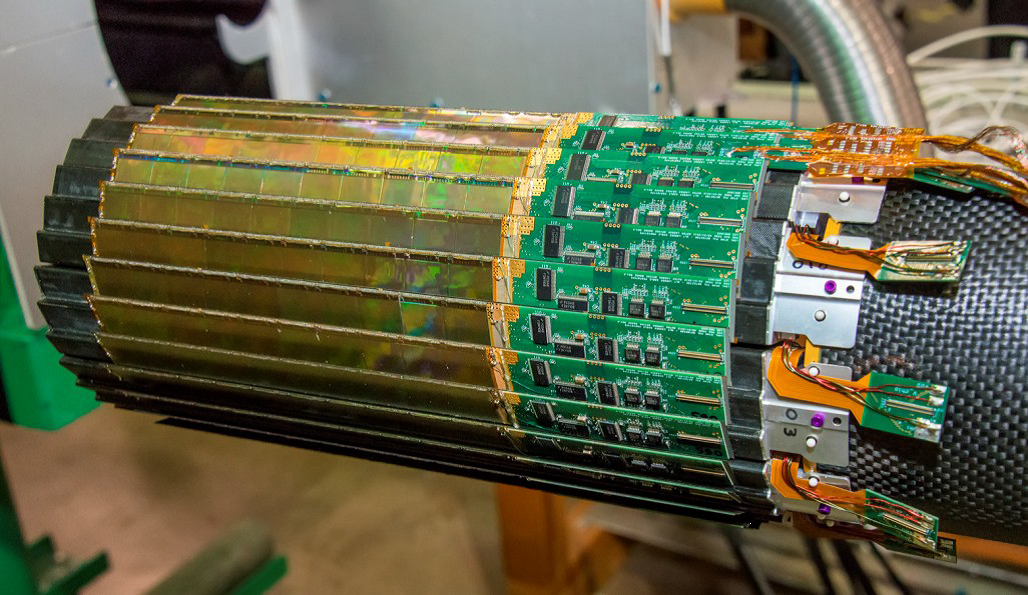
\includegraphics[width=0.6\hsize]{Detector/fig/VTX_STAR.png}
\caption{The vertex detector of the STAR experiment based on the "ULTIMATE" CMOS pixel sensor.}
\label{fig:det:VTX_STAR}
\end{figure}

\subparagraph*{\bf DEPFET sensors: }

The development of DEPFET sensors in particle physics is reaching maturity. Following the demonstration of small
prototypes~\cite{Andricek:2011zza,Velthuis:2008zza} and first operational ladders five years ago the technology was 
chosen as the baseline for the vertex detector~\cite{Marinas:2011zz} of the Belle II experiment~\cite{Abe:2010gxa}. 
As many requirements of Belle II are similar to those
of the ILC, this can be seen as a 30\% prototype of the ILC vertex detector. DEPFET ladders have been successfully used 
in the BELLE II beam commissioning detector (BEAST 2). The first layer of the pixel vertex detector was installed in 2018
and is now in operation in the experiment (Figure~\ref{fig:det:VTX_BELLE2} bottom). Due to a low yield of the module assembly 
process, the second layer vertex detector is expected to be completed in 2020. While the experiment is 
taking data, studies towards future BELLE II upgrades based on advanced DEPFET technology are starting. The development of advanced DEPFET solutions for the ILD vertex detector is synergetic with this effort.

\begin{figure}[t!]
\centering
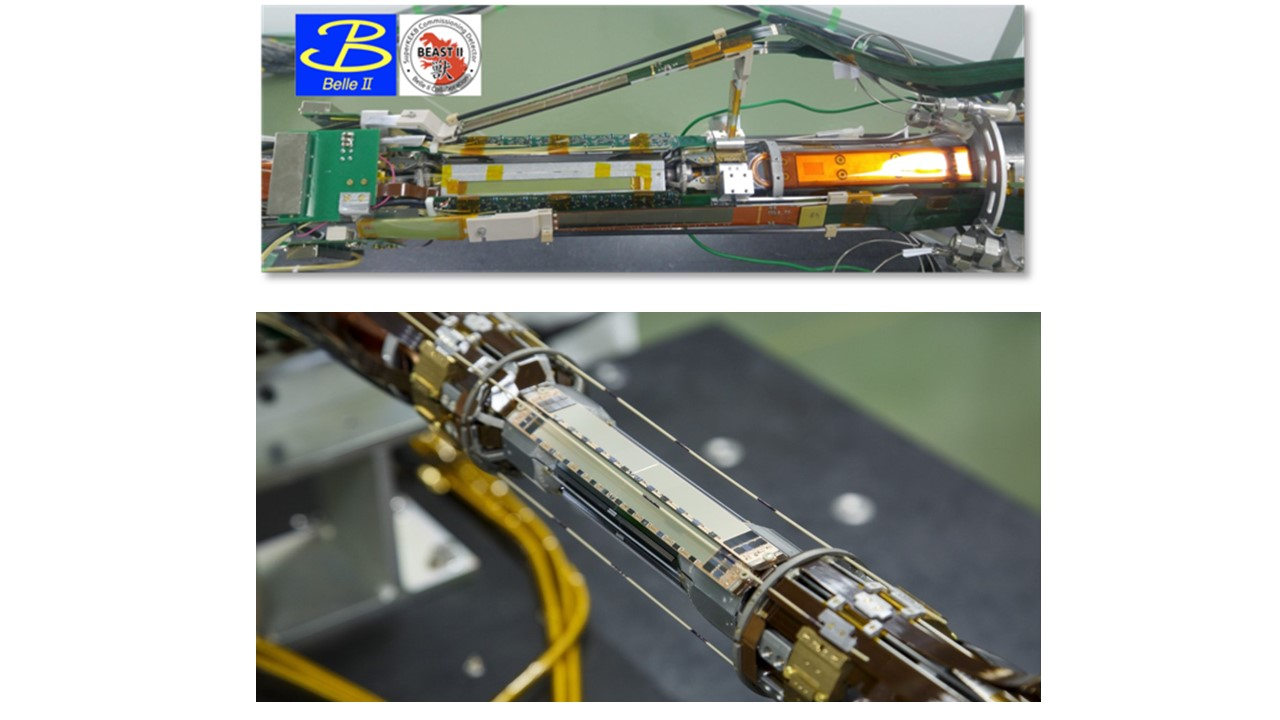
\includegraphics[width=1.0\hsize]{Detector/fig/VTX_BELLE2.jpg}
\caption{Pixel detectors of the BELLE II experiment. Top: beam commissioning with "PLUME" CMOS (inclined sensors) and DEPFET (barrel) ladders. Bottom: the BELLE II DEPFET vertex detector.}
\label{fig:det:VTX_BELLE2}
\end{figure}

\subparagraph*{\bf FPCCD sensors: }

The FPCCD technology is not yet used in full size detector applications but a first large prototype has been built [ref] with a sufficient size to cover the inner layer of the ILD vertex detector. The prototype is currently undergoing detailed characterization with e.g. radioactive source signals (Figure~\ref{fig:det:VTX_FPCCD}). Irradiation tests of FPCCDs are also being performed since radiation hardness is a critical aspect of this technology.   

\begin{figure}[t!]
\centering
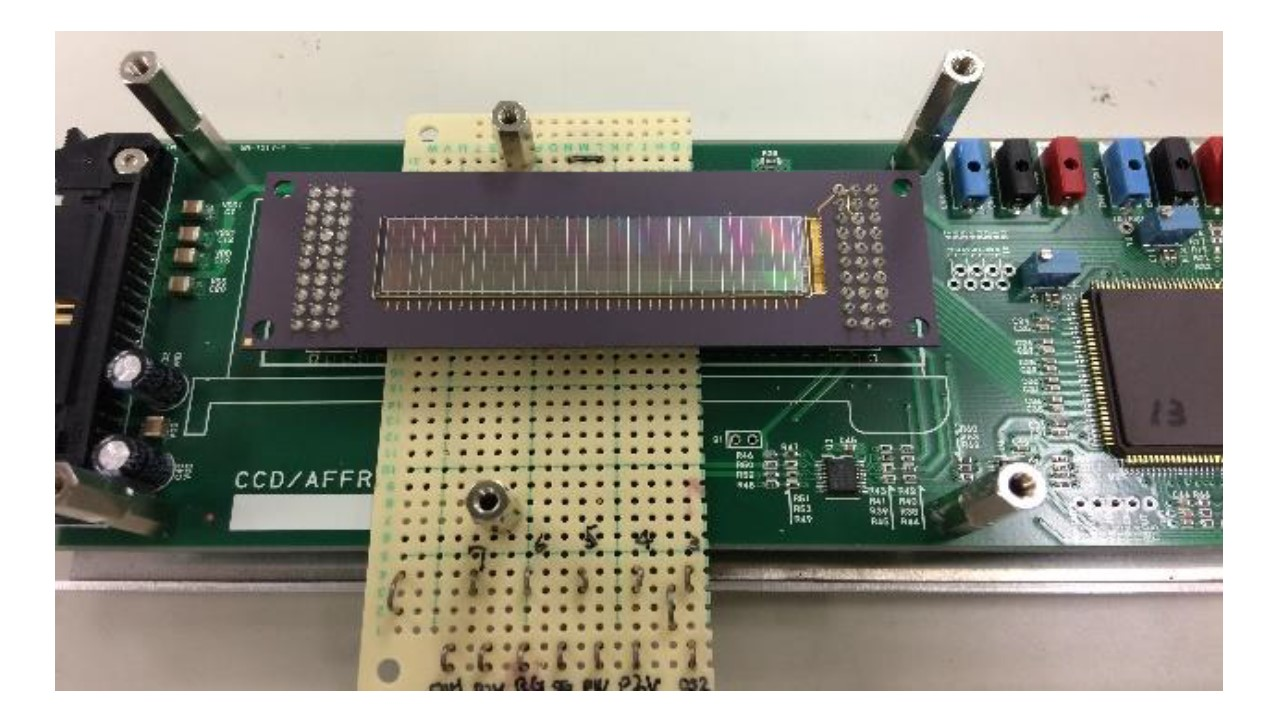
\includegraphics[width=0.6\hsize]{Detector/fig/VTX_FPCCD.jpg}
\caption{First full size FPCCD ladder on its test bed.}
\label{fig:det:VTX_FPCCD}
\end{figure}

\vspace{2cm}